\documentclass{jarticle}
\usepackage[dvipdfmx]{graphicx}
\usepackage{here}
\title{前期個人開発企画書}
\author{6119019056 山口力也}
\date{2019/06/24日提出}


\begin{document}
\maketitle
\section{ゲーム内容}
\subsection{概略}
本ゲームは,2Dのシューティングゲームである.プレイヤーは弾丸を用いて敵機を撃ち落としながら進んでいきボスを倒せばクリアとなる.ただし普通のシューティングゲームと違い,プレイ中に4択のクイズが出題され,その問題に正解しなければゲームオーバーとなる. \\
以下表\ref{table:gamenaiyou}にゲーム内容の詳細を示す.
\begin{table}[H]
\caption{ゲーム内容}
		\begin{tabular}{c}
		\label{table:gamenaiyou}
			%1 
			\begin{minipage}{0.5\hsize}
				\begin{center}
					\begin{tabular}{|p{2.4cm}p{2.4cm}|} \hline
					ゲームジャンル: & シューティングゲーム \\
					プレイヤー人数: & 1人 \\ \hline
					\end{tabular}
				\end{center}
			\end{minipage}
			%2
			\begin{minipage}{0.5\hsize}
				\begin{center}
					\begin{tabular}{|p{2.4cm}p{2.4cm}|} \hline
					ゲームに対するルール & 1.敵機の弾丸が当たったら終了 \\ 
												& 2.クイズが不正解だったら終了 \\ \hline
					\end{tabular}
				\end{center}
			\end{minipage}
		\end{tabular}
\end{table}

\subsection{コンセプト}
誰もが直感的にわかる操作方法になるように工夫する.また難易度設定を導入することで,初心者から上級者まで楽しめるようにすることを目標とする.

\subsection{操作方法}
ゲームの入力用デバイスとしてはジョイパッドを用いる.詳細なキーと動作を以下表\ref{table:inputdevice}を示す.

\begin{table}[H]
\caption{キー入力と動作}
	\begin{center}
		\begin{tabular}{|c|c|}\hline \hline
		キー入力 & 動作 \\ \hline
		上矢印キー & 上方向に動く \\ 
		下矢印キー & 下方向に動く \\ 
		右矢印キー & 右方向に動く \\ 
		左矢印キー & 左方向に動く \\ 
		R1キー & 弾丸発射 \\
		四角キー & 解答を選択(1) \\ 
		三角キー & 解答を選択(2) \\
		丸キー & 解答を選択(3) \\
		バツキー & 解答を選択(4) \\ \hline
		\end{tabular}
	\end{center}
\label{table:inputdevice} 
\end{table}

\section{実装方法}
\subsection{データの構造}
以下表\ref{table:data}に主なデータの構造を示す.

\begin{table}[H]
\caption{共通の構造}
	\begin{center}
		\begin{tabular}{|c|c|c|}\hline 
		データ型& 変数名 & 内容 \\ \hline
		int & type &オブジェクトの型(プレイヤー,敵,弾,etc) \\ 
		Point &pos & オブジェクトの座標 \\
		unsigned short & id & オブジェクトの番号 \\ 
		\hline
		\end{tabular}
	\end{center}
\label{table:data} 
\end{table}

以下表\ref{table:player}にプレイヤー固有の構造体を示す.
\begin{table}[H]
\caption{キャラ固有の構造}
	\begin{center}
		\begin{tabular}{|c|c|c|}\hline 
		データ型& 変数名 & 内容 \\ \hline
		unsigned short & hp & キャラのhp \\ 
		int &status &キャラの状態  \\
		\hline
		\end{tabular}
	\end{center}
\label{table:player} 
\end{table}

クイズの構造はまだ考えれていないので,まずはシューティングゲームの基本的な枠組みができた後,クイズの方を作成していきたいと思う.

\section{ガントチャート}
以下図\ref{fig:gantt}にガントチャートの図を示す.

\begin{figure}[H]
\begin{center}
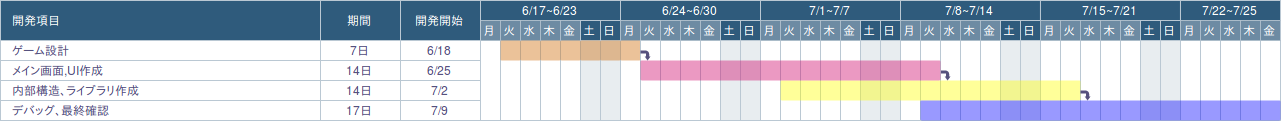
\includegraphics[width=7.0cm]{chart.png}
\caption{ガントチャート図}
\label{fig:gantt}
\end{center}
\end{figure}


\end{document}
